%%%%%%%%%%%%%%%%%%%%%%%%%%%%%%%%%%%%%%%%%
% LaTeX Template
% Version 1.0 (5/5/12)
%
% This template has been downloaded from:
% http://www.LaTeXTemplates.com
%
% Original author:
% Frits Wenneker (http://www.howtotex.com)
%
% License:
% CC BY-NC-SA 3.0 (http://creativecommons.org/licenses/by-nc-sa/3.0/)
%
%%%%%%%%%%%%%%%%%%%%%%%%%%%%%%%%%%%%%%%%%

%----------------------------------------------------------------------------------------
%	PACKAGES AND OTHER DOCUMENT CONFIGURATIONS
%----------------------------------------------------------------------------------------

\documentclass[paper=a4, fontsize=12pt]{scrartcl} % A4 paper and 11pt font size

\usepackage[T1]{fontenc} % Use 8-bit encoding that has 256 glyphs
%\usepackage{fourier} % Use the Adobe Utopia font for the document - comment this line to return to the LaTeX default
\usepackage[english]{babel} % English language/hyphenation
\usepackage{amsmath,amsfonts,amsthm,amssymb} % Math packages
\usepackage{mathtools}

\usepackage{multicol}
\usepackage{relsize}
\usepackage{graphicx}
\usepackage{float}

\usepackage{enumitem}
\usepackage{gensymb}
\usepackage{textcomp}
\usepackage{csquotes}
\usepackage{setspace}
\usepackage[ruled,vlined]{algorithm2e}

\usepackage[colorlinks = true,
            linkcolor = black,
            urlcolor  = blue,
            citecolor = red,
            anchorcolor = blue]{hyperref}

\usepackage{sectsty} % Allows customizing section commands
\allsectionsfont{\centering \normalfont\scshape} % Make all sections centered, the default font and small caps

\usepackage{fancyhdr} % Custom headers and footers
\pagestyle{fancyplain} % Makes all pages in the document conform to the custom headers and footers
%\fancyhead{} % No page header - if you want one, create it in the same way as the footers below
%\fancyfoot[L]{} % Empty left footer
%\fancyfoot[C]{} % Empty center footer
\fancyfoot[R]{\thepage} % Page numbering for right footer
\renewcommand{\headrulewidth}{0pt} % Remove header underlines
\renewcommand{\footrulewidth}{0pt} % Remove footer underlines
\setlength{\headheight}{13.6pt} % Customize the height of the header

\numberwithin{equation}{section} % Number equations within sections (i.e. 1.1, 1.2, 2.1, 2.2 instead of 1, 2, 3, 4)
\numberwithin{figure}{section} % Number figures within sections (i.e. 1.1, 1.2, 2.1, 2.2 instead of 1, 2, 3, 4)
\numberwithin{table}{section} % Number tables within sections (i.e. 1.1, 1.2, 2.1, 2.2 instead of 1, 2, 3, 4)

\setlength{\parindent}{0pt} % Removes all indentation from paragraphs - comment this line for an assignment with lots of text
\setlength{\parskip}{1em}

%----------------------------------------------------------------------------------------
%	TITLE SECTION
%----------------------------------------------------------------------------------------

\newcommand{\horrule}[1]{\rule{\linewidth}{#1}} % Create horizontal rule command with 1 argument of height

\title{	
    \normalfont \normalsize 
    \horrule{3pt} \\[0.4cm] % Thin top horizontal rule
    \LARGE \textbf{Deep Learning: A Mathematical Overview} \\[0.1cm] % The assignment title
    \horrule{1pt} \\[0.5cm] % Thick bottom horizontal rule
}

\author{
    \footnotesize \textbf{Anne Gelb} \\[-0.3cm]
    \footnotesize Mathematics \\[-0.3cm]
    \footnotesize Dartmouth College
    \and
    \footnotesize \textbf{Sriram Bapatla} \\[-0.3cm]
    \footnotesize Mathematics \\[-0.3cm]
    \footnotesize Dartmouth College
    \and
    \footnotesize \textbf{Yusuf Olokoba} \\[-0.3cm]
    \footnotesize Computer Sciences \\[-0.3cm]
    \footnotesize Dartmouth College
    \and
    \footnotesize \textbf{Jack Zhang} \\[-0.3cm]
    \footnotesize Mathematics \\[-0.3cm]
    \footnotesize Dartmouth College
} % Your name

\date{\normalsize\today} % Today's date or a custom date

\DeclareMathOperator*{\argmin}{arg\,min}
\DeclareMathOperator*{\argmax}{arg\,max}

\begin{document}

\maketitle % Print the title

%----------------------------------------------------------------------------------------
%	Abstract
%----------------------------------------------------------------------------------------

\section*{Abstract}

In this paper, we perform an overview of deep learning, as it is today, from a mathematical perspective.
We start with the fundamentals of learning, then go on to analyze how different tasks are learnt, what data 
is used to learn such tasks, and how to better understand said data.

This paper is by no means comprehensive, hence we intend it to simply be a high level overview of the [interesting] 
topics that define deep learning.

\pagebreak

%----------------------------------------------------------------------------------------
%	Table of Contents
%----------------------------------------------------------------------------------------

\tableofcontents

\pagebreak

%----------------------------------------------------------------------------------------
%   Neural Networks: An Overview
%----------------------------------------------------------------------------------------

\section{Neural Networks: An Overview}

At the highest level, neural networks function estimators. Given a set of inputs $\{ x_1, \ldots, x_n \}$ and 
a corresponding set of outputs $\{ y_1, \ldots, y_n \}$, a neural network \textit{learns} the model $f(x)$ which 
best approximates the given data $f(x_i) = y_i$.

The simplest neural network to consider is a linear regressor, which learns the $w^*, b^*$ that best 
fits some given linear data $f(x_i) = w^* x_i + b^* = y_i$. Unfortunately, your linear regressor will not spark a revolution 
because most observable data we consider are non-linear. But thankfully with only a few additions, we can in fact build 
highly sophisticated models which learn highly complex relationships in data. To do so, we introduce the \textit{Perceptron}:
\begin{align*}
    f(x) = \sigma(wx + b)
\end{align*}
Where $\sigma$ is the \textit{activation function}, $w$ is the weight, and $b$ is some bias. The activation function $\sigma(\cdot)$ is used to
enable the perceptron to learn non-linear features, depending on the choice of the activation. The rest of the formulation is simply a linear 
regressor.

You might be thinking that a single perceptron would still not be able to learn a large variety of relationships, and you would be correct. Although there 
is active debate on the topic, it has been emperically shown that increasing the number of perceptrons in a model increases its \textit{capacity}\cite{vcdim}, that is 
its ability to learn more complex relationships. Hence, we introduce the Multi-Layer Perceptron (MLP):

\textit{INCOMPLETE}: Add image

The MLP forms the basis of deep neural network topologies. We will discuss two notable topologies: autoencoders and convolutional neural networks.

\pagebreak

\subsection{Autoencoders and Representation Learning}

Autoencoder models are trained in \textit{unsupervised learning tasks}, where the objective is to reproduce some input $\vec{x}$ as closely as possible, using less information
than that of the provided input.

\begin{figure}[H]
    \centering
    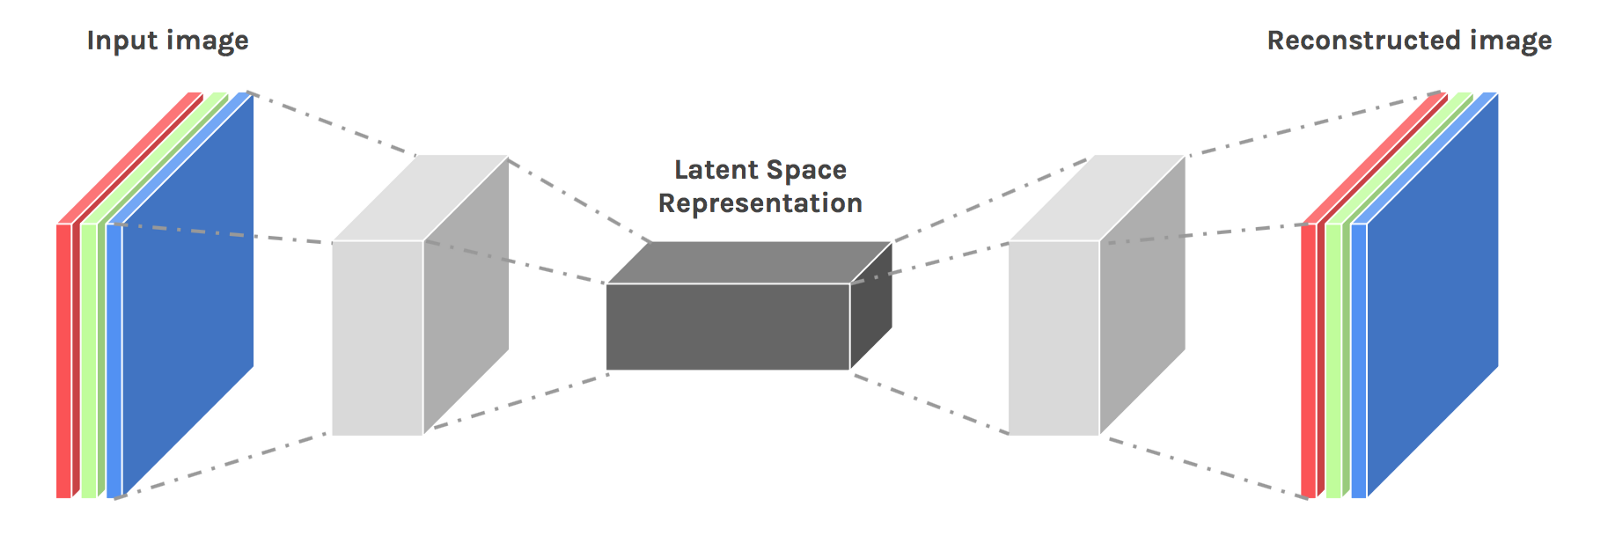
\includegraphics[width=0.8\textwidth]{images/autoencoder}
    \caption{Autoencoder architecture. \href{https://hackernoon.com/autoencoders-deep-learning-bits-1-11731e200694}{Source}}
\end{figure}

An autoencoder is comprised of two sub-networks, an \textit{encoder} which learns a significantly lower-dimensional feature space for its input, and a decoder 
which learns a transformation from the learned feature space back to the input domain, while preserving as much useful information as possible.

One way to consider autoencoders is as a non-linear principal component analysis over the input space. They are extremely useful for compression tasks, but also for 
representation learning.

In representation learning, the task is to learn not only the most defining feature of a given distribution, but also the [principal] factors of 
variation within the distribution. This is extremely useful for generative tasks, where one might want to generate completely new samples by interpolating 
between certain features within the distribution. Disentanglement and causal inference are significant [next steps] in representation learning.

\pagebreak

\subsection{Convolutional Neural Networks}

Convolutional Neural Networks (\textit{CNN} hereafter) are architected for feature extraction from images. Computers store images as stacks
two-dimensional matrices where elements correspond to pixel intensity at their spatial locations within the image. The task of extracting features from 
an image requires special [precautions] due to the fact that certain features, say a cat face, might occur at several distinct regions within 
a given image. Hence the network would require feature extraction units that are spatially-invariant. To do so, we utilize the 
discrete convolution:
\begin{align*}
    I(x, y) * K(\cdot, \cdot) = \sum_{i = 1}^k \sum_{j = 1}^k I(x + i, y + k) * K(k - i, k - j)
\end{align*}
Where $I(x, y)$ is an image indexed at positions $(x, y)$ and $K(\cdot, \cdot)$ is a learned convolution kernel. During training, the CNN learns a series of 
kernels $\{ K_1(\cdot, \cdot), \ldots, K_n(\cdot, \cdot) \}$ which respond to useful features for the task being learnt.

\begin{figure}[H]
    \centering
    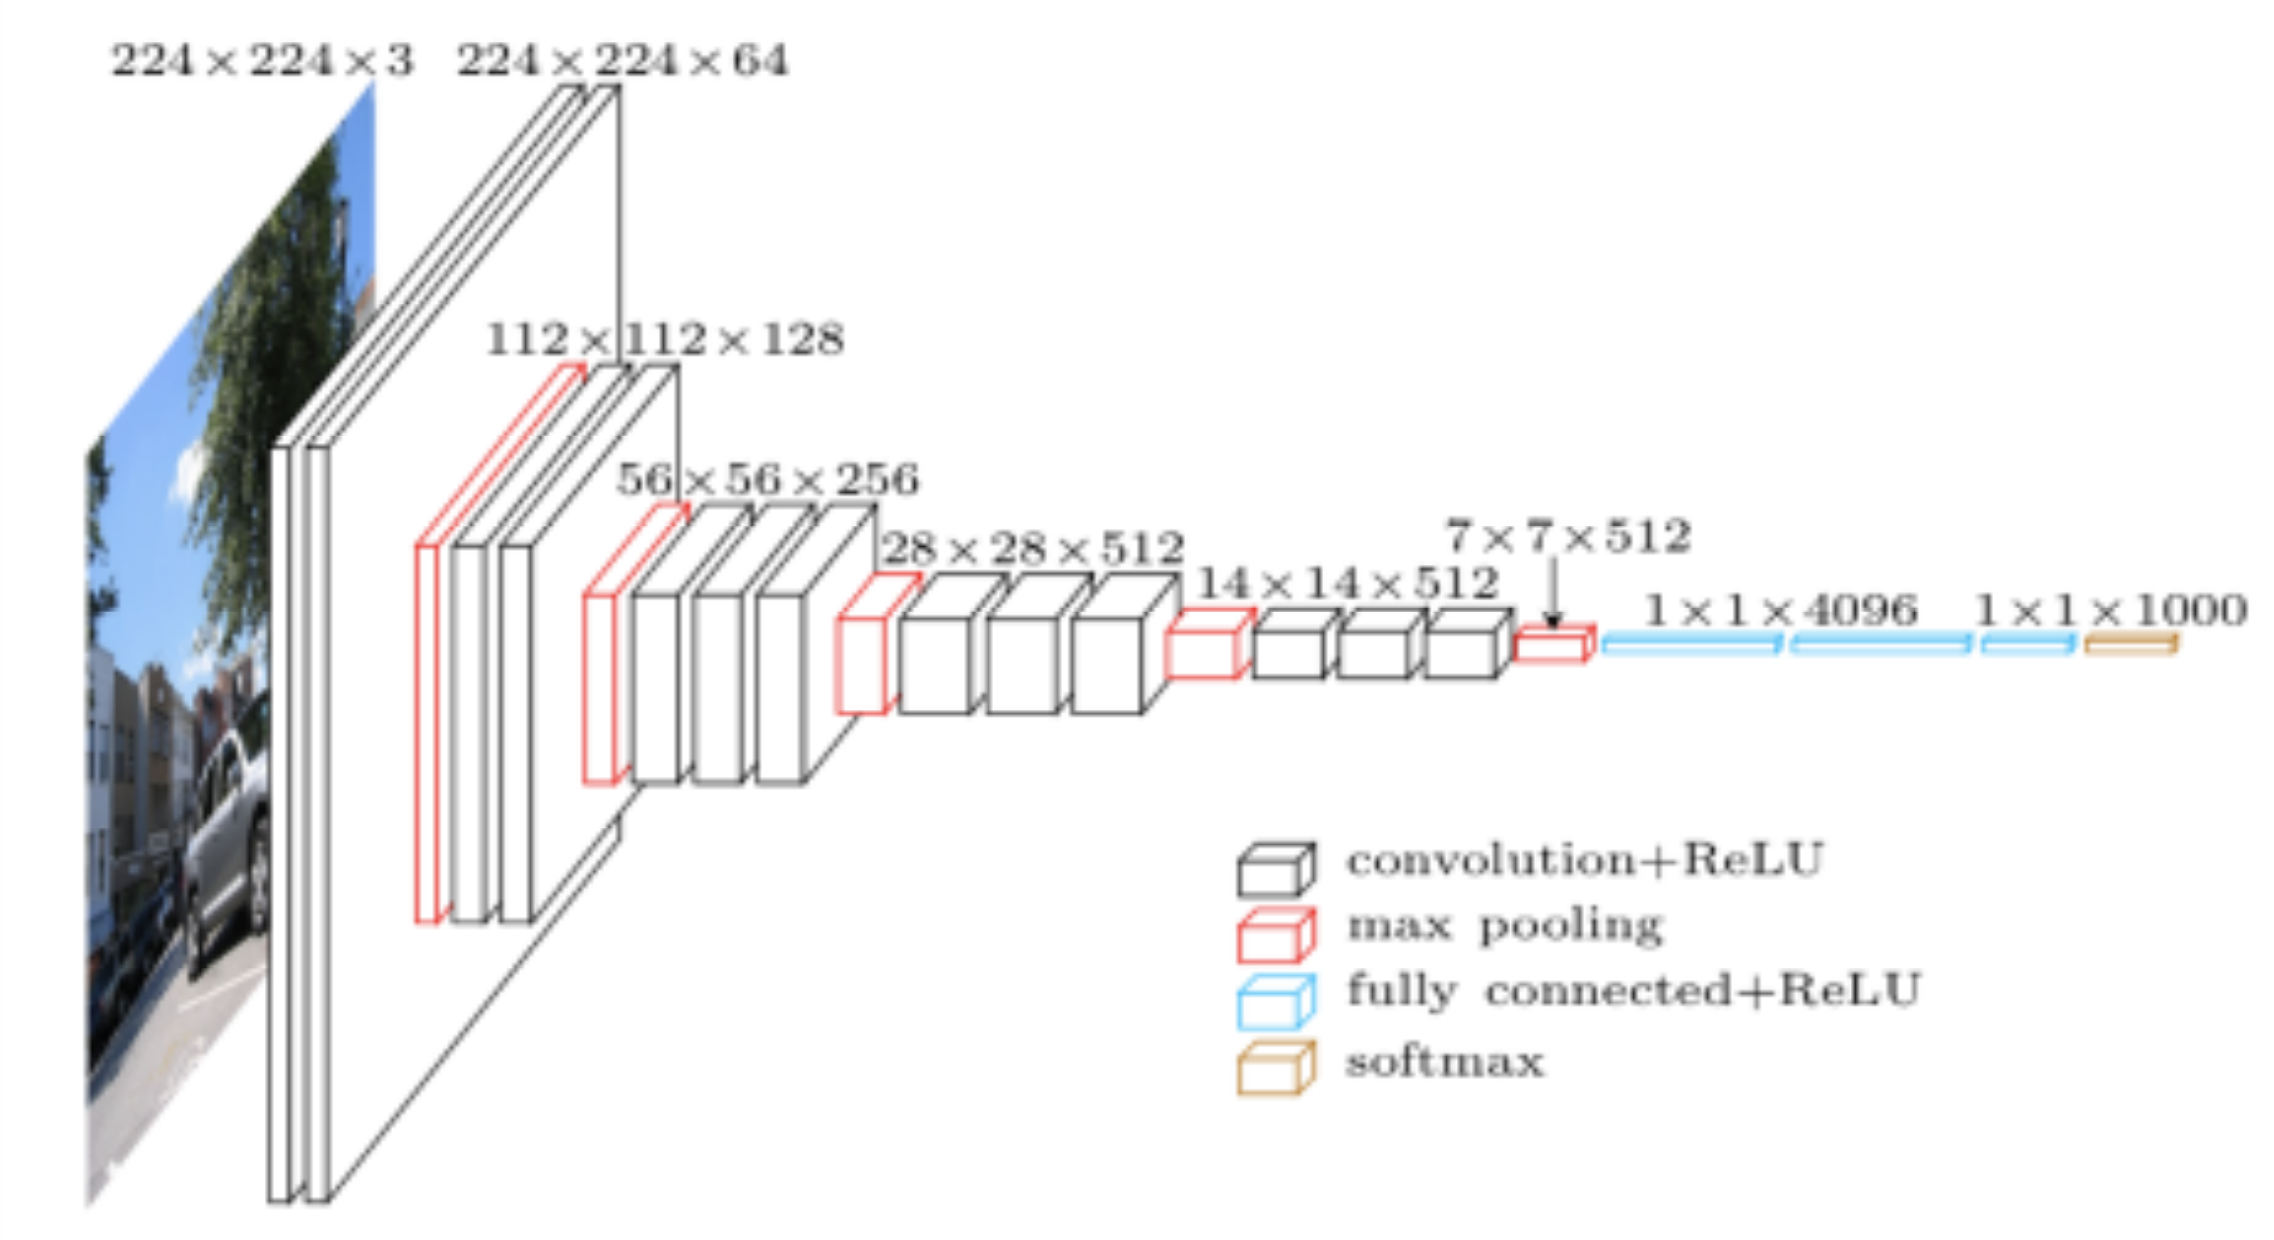
\includegraphics[width=0.65\textwidth]{images/cnn}
    \caption{CNN architecture. \href{https://medium.com/@purnasaigudikandula/a-beginner-intro-to-convolutional-neural-networks-684c5620c2ce}{Source}}
\end{figure}

This design is inspired by the mamallian visual cortex \cite{cortex}, which recognizes features using an ensemble of feature extractors. Earlier kernels learn to recognize 
the simplest features like lines at different orientations whereas later kernels learn more complex representations, like cat faces, as the combinations of the simpler learned kernels.

\subsection{Other Notable Architectures} % RNN, LSTM

Some other notable architectures include Recurrent Neural Networks (RNN) and Long-Short Term Memory (LSTM) models. These architectures are targeted for learning time-series data, where previously-encountered 
data might influence the learnt features of new data. They are usually used for language modeling problems.

\pagebreak

%----------------------------------------------------------------------------------------
%	Learning in Neural Networks
%----------------------------------------------------------------------------------------

\section{Learning in Neural Networks}

Given a neural network and some training data, how does the network learn the data? 
The objective is for the network to learn a model that best fits the data. To reach this objective, we need 
two things: a notion of how well the current model performs (covered in more detail in chapter 3), and a way to tune
the current model based on its evaluated performance to yield some new model. The latter problem falls into the 
broad category of numerical optimization methods.

%----------------------------------------------------------------------------------------
%	1st Order Optimization
%----------------------------------------------------------------------------------------

\subsection{1st Order Optimization}

Consider an arbitrary neural network $f(\vec{p})$ with of $n$ parameters which is trained to produce outputs $\hat{y}$ that minimize some cost function $C(\vec{p})$:
\begin{align*}
    \hat{y} &= f(\vec{p}) \\
    C(\vec{p}) &= | \hat{y} - y |
\end{align*}
Our model learns the parameters $\vec{p} = \{ w_1, b_1, \ldots \}$ which defines a model that best fits the given data $\{ y_1, y_2, \ldots \}$. We wish to iteratively update $\vec{p}$
to minimize $C(\vec{p})$. Taking a first order Taylor expansion of $C$ at $\vec{p}$, we can estimate $C(\vec{p} + \Delta \vec{p})$ for a small perturbation $\Delta \vec{p}$:
\begin{align*}
    C(\vec{p} + \Delta \vec{p}) &\approx C(\vec{p}) +  \Delta \vec{p}^T \nabla C(\vec{p}) \\
    \nabla C(\vec{p}) &= \left[ \frac{\delta C(\vec{p})}{\delta \vec{p}_1}, ..., \frac{\delta C(\vec{p})}{\delta \vec{p}_s} \right]^T
\end{align*}

Hence:
\begin{align*}
    C(\vec{p} + \Delta \vec{p}) < C(\vec{p}) \mathrm{\ if\ } \Delta \vec{p}^T \nabla C(\vec{p}) < 0
\end{align*}

It is apparent that $\Delta \vec{p} \cdot \nabla C(\vec{p})$ is maximized when $\Delta p = \nabla C(\vec{p})$. Hence we arrive at the 
gradient descent update scheme:
\begin{align*}
    \vec{p}^{(i+1)} = \vec{p}^{(i)} - \eta \nabla C(\vec{p})
\end{align*}
We call $\eta$ the \textit{learning rate}, and keep it at a small value since we are merely approximating $\nabla C$.

\pagebreak

\subsubsection{Backpropagation}

Given the gradient descent update scheme, we need to compute $\nabla C(\vec{p})$. Due to the topology of the neural network, we can analytically compute it. Consider a toy artificial neural network,
$N = \{a^{(1)}, \ldots, a^{(L)} \}, \forall a^{(i)} \in N, a^{(i)} \in \mathbb{R}$. At each layer, we have:
\begin{align*}
    a^{(i)} &= \sigma^{(i)} (z^{(i)}) \\
    z^{(i)} &= w^{(i)} a^{(i - 1)}
\end{align*}
Where $\sigma^{(i)}$ is an activation function, usually one of $tanh$, $sigmoid$, $ReLU$, $softmax$, and so on. We ignore the bias term for illustration purposes. Now suppose we train our network on a single example $y$, we have:
\begin{align*}
    C &= | a^{(L)} - y | \\
    \frac{\delta C}{\delta w^{(L)}} &= \frac{\delta C}{\delta a^{(L)}} \cdot \frac{\delta a^{(L)}}{\delta z^{(L)}} \cdot \frac{\delta z^{(L)}}{\delta w^{(L)}} \\
    \frac{\delta C}{\delta w^{(L - 1)}} &= \frac{\delta C}{\delta a^{(L)}} \cdot \frac{\delta a^{(L)}}{\delta z^{(L)}} \cdot \frac{\delta z^{(L)}}{\delta a^{(L - 1)}} \cdot \frac{\delta a^{(L - 1)}}{\delta z^{(L - 1)}} \cdot \frac{\delta z^{(L - 1)}}{\delta w^{(L - 1)}} \\
    &... \\
    \frac{\delta C}{\delta w^{(1)}} &= \frac{\delta C}{\delta a^{(L)}} \cdot \frac{\delta a^{(L)}}{\delta z^{(L)}} \cdot \frac{\delta z^{(L)}}{\delta a^{(L - 1)}} \cdot \ldots \cdot \frac{\delta z^{(2)}}{\delta a^{(1)}} \cdot \frac{\delta a^{(1)}}{\delta z^{(1)}} \cdot \frac{\delta z^{(1)}}{\delta w^{(1)}}
\end{align*}
As we continue to unwind this, we work our way backward from the output layer $a^{(L)}$ to the input layer $a^{(1)}$. This defines the backpropagation technique to compute $\nabla C(\vec{p})$.

Scaling this up to several input samples $\{y_1, ..., y_n\}$ simply involves avergaing the computed gradients over each $y_i$. Similarly, scaling this 
to fully connected networks (FCN) involves taking the sum of the computed partials over each input neuron. Consider a neuron $i$ in a given layer $l$, $a^{(l)}_i$. We have:
\begin{align*}
    \frac{\delta C}{\delta a^{(l)}_k} &= \sum_{j = 1}^{n_L} \frac{\delta C}{\delta a^{(l+1)}_j} \cdot \frac{\delta a^{(l+1)}_j}{\delta z^{(l+1)}_j} \cdot \frac{\delta z^{(l+1)}_j}{\delta a^{(l)}_k} 
\end{align*}
Special care must be taken when choosing an activation function $\sigma^{(i)}$, because:
\begin{align*}
    \frac{\delta a^{(l)}}{\delta z^{(l)}} = \sigma'(z^{(l)})
\end{align*}
Now consider the \href{https://www.desmos.com/calculator/esp2zr8pgp}{$tanh$} and \href{https://www.desmos.com/calculator/kn9tpwdan5}{$sigmoid$} activation functions. They have a desirable property in that they 
\textit{squish} their activations to a predictable range, and their gradients around the origin are also of reasonable magnitude. The problem is that at extrema, these 
activations produce gradients with magnitude $\approx 0$. It becomes apparent from the above equations that once this happens, the model becomes unable to learn as no gradient magnitude gets 
backpropagated to earlier layers.

Nowadays, we tend to use Parametric Rectified Linear Unit (PRELU) activation which has a fixed negative gradient:
\begin{align*}
    \sigma(x) = \left.
        \begin{cases}
            x & \text{when } x \geq 0 \\
            \alpha x & \text{otherwise}
        \end{cases}
    \right\} \\
    \sigma'(x) = \left.
        \begin{cases}
            1 & \text{when } x \geq 0 \\
            -\alpha & \text{otherwise}
        \end{cases}
    \right\}
\end{align*}

And in order to retain the nice property of reasonable gradient magnitudes that $sigmoid$ and $tanh$ have, we 
introduce layers that normalize the activations over a batch \cite{batchnorm} or instance \cite{instancenorm} to have a given or learned mean and standard deviation.

Another problem similar to vanishing gradients is exploding gradients. This is usually as a result of training data with skewed covariance. We usually preprocess 
training data to have a zero mean and unit standard deviation. There are also training techniques that impose a gradient penalty when computing training losses \cite{wgangp}.

%----------------------------------------------------------------------------------------
%	1st Order Update Schemes
%----------------------------------------------------------------------------------------

\subsection{1st Order Update Schemes}

We have seen the mathematical formulations of gradient descent as it relates to ANN's. Now we will consider the practical implications of the vanilla implementation, and how
these implications inform different first order update schemes that are used in the field today.

We begin with gradient descent, which we will refer to as full-batch gradient descent. In this algorithm, we compute the gradient of the loss landscape $\nabla C(\vec{p})$ by averaging 
contributions over all $n$ samples of our training data $D, |D| = n$. Considering that we now train models with hundreds of thousands and millions of data samples, performing 
a single step of the full-batch gradient descent becomes computationally intractable given current hardware limitations. A healthy compromise is to perform each gradient descent step
over a randomly selected mini-batch $B \subset D, |B| << |D|$. This forms the basis of Stochastic Gradient Descent.

\subsubsection{Stochastic Gradient Descent}

Given a dataset $D$ such that $|D| = n$, we choose a random minibatch $B$ with $|B| = m$. We then perform gradient descent with this minibatch:
\begin{align*}
    C(\vec{p}) &= \frac{1}{m} \sum_{i=1}^m |\hat{y}_i - y_i| \\
    \vec{p}^{(i+1)} &= \vec{p}^{(i)} - \frac{\eta}{m} \sum_{i=1}^m \nabla C_i(\vec{p})
\end{align*}

In practice, SGD has a number of interesting properties. Because of its stochasticity its gradient updates tend to be noisy, even though they generally reach the same minimums. This noise is 
often a feature rather than a bug: when the optimizer reaches a sharp local minimum, the noise allows it to escape this minimum. Unfortunately, SGD is not very robust against 
saddle points. A saddle point is a region with near-zero gradients, but one which isn't a minimum. In regions like this, the optimizer will slow down to a halt since $\nabla C(\vec{p}) \approx \vec{0}$.

\subsubsection{Momentum and Nesterov Momentum}

We make a modification to the SGD algorithm to add a \textit{momentum} term. Conceptually, one could imagine the optimizer as a ball on the 
optimization landscape. Its motion at a given update becomes defined not only by the gradient of the hypersurface beneath it, but by its velocity up to that point. Hence we have the update 
scheme for SGD+Momentum:
\begin{align*}
    \vec{p}^{(t+1)} &= \vec{p}^{(t)} - \vec{v}^{(t+1)} \\
    \vec{v}^{(t+1)} &= \beta \vec{v}^{(t)} + \eta \nabla C(\vec{p}^{(t)})
\end{align*}
$\beta$ is a hyperparameter, usually chosen to be $0.9$ or $0.99$. The momentum term allows the optimizer to escape local minima and saddle points, as it has `inertia'.

\textit{INCOMPLETE}. Nesterov momentum and comparison image.

\subsubsection{Adaptive Sub-Gradient}

Now consider another challenge for the optimizer. On some loss landscapes, the gradients in one axis could be significantly higher in magnitude than in other axes. This is conceptually similar to an ill-conditioned 
matrix in linear algebra, which is defined by a large ratio between its largest and smallest eigenvalues. On such a hypersurface, SGD will oscillate significantly on the more-skewed axis and move very slowly on the less-skewed axis.

A natural way to prevent this is to keep a per-parameter learning rate, $\eta_i$. The Adagrad optimizer computes its per-parameter learning rate by dividing the nominal learning rate by the rolling sum of all 
past gradients for a given parameter:
\begin{align*}
    \eta^{(t+1)}_i &= \frac{\eta}{\sqrt{\sum_{s=1}^t \left(\nabla C(\vec{p})^{(s)}_i \right)^2}} \\
    \vec{p}^{(t+1)} &= \vec{p}^{(t)} - \left(\vec{\eta}^{(t+1)}\right)^T \nabla C(\vec{p}^{(t)})
\end{align*}

\subsubsection{Root Mean Square Propagation}

The obvious problem with this scheme is that as the optimizer steps increase, the learning rate becomes smaller and smaller. As a result, the RMSProp update rule is proposed which linearly decays the dividend with some $\beta$ hyperparameter.

\textit{INCOMPLETE}. Equation here.

\subsubsection{Adpative Moment Estimation}

The Adaptive Moment Estimation (Adam) optimizer, which is the most commonly used optimizer, combines SGD+Momentum and RMSProp to compute a 
per-parameter learning rate augmented with a velocity term:

\textit{INCOMPLETE}. Equation here.

\pagebreak

%----------------------------------------------------------------------------------------
%	2nd Order Optimization
%----------------------------------------------------------------------------------------

\subsection{2nd Order Optimization}

The gradient descent method finds the minimum of a given function by taking steps that minimize the first order Taylor 
approximation of the given function. What if we could construct a better approximation of the given function? To do so, we could use the 
second order Taylor approximation:
\begin{align*}
    f(\vec{x} + \Delta \vec{x}) \approx &f(\vec{x}) + \Delta \vec{x}^T \nabla f(\vec{x}) + \frac{1}{2} \Delta \vec{x}^T \nabla^2 f(\vec{x}) \Delta \vec{x}
\end{align*}

Hence we expect to minimize this approximation with respect to $\Delta \vec{x}$ when:
\begin{align*}
    \frac{\delta f(\vec{x} + \Delta \vec{x})}{\delta \Delta \vec{x}} = \nabla f(\vec{x}) + \nabla^2 f(\vec{x}) \Delta \vec{x} = 0
\end{align*}

This gives us an update scheme for our optimization:
\begin{align*}
    \Delta \vec{x} = \vec{x}_{(k+1)} - \vec{x}_{(k)} &= - H^{-1}_{(k)} \nabla f(\vec{x}_{(k)}) \\
    \therefore \vec{x}_{(k+1)} &= \vec{x}_{(k)} - H^{-1}_{(k)} \nabla f(\vec{x}_{(k)}) \\
    \text{where } H_{(k)} &= \nabla^2 f(\vec{x}_{(k)})
\end{align*}

This defines \textbf{Newton's Method} used for root finding. It is worth noting that we can only expect this method to converge when the Hessian 
is positive definite. Suppose we have chosen some $\vec{x}$ such that $\nabla f(\vec{x}) \approx 0$. At one such critical point, our approimation becomes:
\begin{align*}
    f(\vec{x} + \Delta \vec{x}) &= f(\vec{x}) + \frac{1}{2} \Delta \vec{x}^T \nabla^2 f(\vec{x}) \Delta \vec{x} \\
    \therefore f(\vec{x} + \Delta \vec{x}) - f(\vec{x}) &= \frac{1}{2} \Delta \vec{x}^T \nabla^2 f(\vec{x}) \Delta \vec{x}
\end{align*}

It becomes apparent that for convergence, it must be the case that $\forall \Delta \vec{x}, f(\vec{x} + \Delta \vec{x}) - f(\vec{x}) > 0$. Hence the need for $H$ to be positive definite.
In practice however, we often cannot guarantee $H$ being positive definite, so instead we construct a surrogate Hessian $G$ for which we can guarantee positive definiteness. We 
do so by ensuring that $\forall \lambda_i \in \lambda(G), \lambda_i > 0$. Let $\vec{v}_i \in \mathbb{R}^n, H\vec{v}_i = \lambda_i \vec{v}_i$ be 
an eigenvector of $H$. We can define $G = (H + \mu I)$ so that:
\begin{align*}
    G\vec{v}_i &= (H + \mu I)\vec{v}_i \\
    &= H\vec{v}_i + \mu I \vec{v}_i \\
    &= \lambda_i \vec{v}_i + \mu \vec{v}_i \\
    &= (\lambda_i + \mu) \vec{v}_i
\end{align*}

Hence with $\mu >> 0$, we can almost guarantee that $G$ is positive definite. This defines the \textbf{Levenberg-Marquadt Modification} used to \textit{dampen} the Hessian. Finally, 
it is worth noting that the Hessian has the nice propery of being able to step directly to the minimum of a quadratic function. Consider the function:
\begin{align*}
    f(\vec{x}) &= \frac{1}{2} \vec{x}^T Q \vec{x} - \vec{x}^T \vec{b} \\
    f'(\vec{x}) &= Q \vec{x} - \vec{b} \\
    f''(\vec{x}) &= Q
\end{align*}

Assuming that $Q = Q^T$ and $\exists \ Q^{-1}$, then Newton update gives:
\begin{align*}
    \vec{x}_{(1)} &= \vec{x}_{(0)} - Q^{-1} \left[ Q\vec{x}_{(0)} - \vec{b} \right] \\
    &= \vec{x}_{(0)} - \vec{x}_{(0)} + Q^{-1} \vec{b} \\
    &= Q^{-1} \vec{b}
\end{align*}

\subsubsection{Symmetric Rank 1 Update}

When optimizing in a small class of problems, like in dynamic simulations with negligible stochasticity, we might be able to analytically compute the Hessian. But in 
most practical problems, it is either impractical or impossible to compute the Hessian, talkless of its inverse. Thankfully, this should not prevent us from taking advantage of 2nd order 
information about $f(\vec{x})$. Indeed, we can approximate the Hessian from previous update steps. This forms the basis of \textbf{Quasi-Newton Methods}. First, we define some terms:
\begin{align*}
    \vec{y}_{(k+1)} &= \nabla f(\vec{x}_{(k+1)}) - \nabla f(\vec{x}_{(k)}) \\
    \Delta \vec{x}_{(k+1)} &= \vec{x}_{(k+1)} - \vec{x}_{(k)}
\end{align*}

We wish to iteratively compute $H$ (or its inverse). We will do so in two steps: first we create an initial estimate; then we will iteratively update the estimate as we take steps. 
A good property to impose on $H$ is that its gradients agree with $f$ at $\vec{x}_{(k+1)}$ and $\vec{x}_{(k)}$:
\begin{align*}
    \nabla f(\vec{x}_{(k)}) &= H \vec{x}_{(k)} \\
    \nabla f(\vec{x}_{(k + 1)}) &= H \vec{x}_{(k + 1)} \\
    \therefore f(\vec{x}_{(k + 1)}) - f(\vec{x}_{(k)}) &= H \vec{x}_{(k + 1)} - H \vec{x}_{(k)} \\
    \vec{y}_{(k+1)} &= H \Delta \vec{x}_{(k+1)}
\end{align*}

This is the \textbf{Secant Condition}. Hence if we take $n$ steps, each in a direction that is linearly-independent from the others, we have:
\begin{align*}
    \begin{bmatrix}
        \vec{y}_1 & \ldots & \vec{y}_n
    \end{bmatrix} = H \begin{bmatrix}
        \Delta \vec{x}_1 & \ldots & \Delta \vec{x}_n
    \end{bmatrix}
\end{align*}

Then $H$ is uniquely determined as $\left[ \Delta \vec{x}_1 \ldots \Delta \vec{x}_n \right]$ must be invertible:
\begin{align*}
    H = \begin{bmatrix}
        \vec{y}_1 & \ldots & \vec{y}_n
    \end{bmatrix} \begin{bmatrix}
        \Delta \vec{x}_1 & \ldots & \Delta \vec{x}_n
    \end{bmatrix}^{-1} \\
    \begin{bmatrix}
        \Delta \vec{x}_1 & \ldots & \Delta \vec{x}_n
    \end{bmatrix} = H^{-1} \begin{bmatrix}
        \vec{y}_1 & \ldots & \vec{y}_n
    \end{bmatrix}
\end{align*}

This defines the initial approximation of the Hessian inverse:
\begin{align}
    \Delta \vec{x}_{(k)} = H_{(k)}^{-1} \vec{y}_{(k)}
\end{align}

For the iterative update, we wish to find a $H_{(k+1)}^{-1}$ that satisfies the above equation. To do so, we consider performing a symmetric rank one update on $H_{(k)}^{-1}$:
\begin{align}
    H_{(k+1)}^{-1} = H_{(k)}^{-1} + \alpha_{(k)} \vec{z}_{(k)} \vec{z}_{(k)}^T
\end{align}

Hence from equation (2.1):
\begin{align*}
    \Delta \vec{x}_{(k)} &= H_{(k+1)}^{-1} \vec{y}_{(k)} \\
    &= \left[ H_{(k)}^{-1} + \alpha_{(k)} \vec{z}_{(k)} \vec{z}_{(k)}^T \right] \vec{y}_{(k)} \\
    \Delta \vec{x}_{(k)} &= H_{(k)}^{-1} \vec{y}_{(k)} + (\alpha_{(k)} \vec{z}_{(k)} \vec{z}_{(k)}^T) \vec{y}_{(k)} \\
    \text{but } \vec{a} \vec{a}^T \vec{b} &\equiv (\vec{a} \cdot \vec{b}) \vec{a} \equiv \vec{a}^T \vec{b} \vec{a}
\end{align*}

So:
\begin{align}
    \Delta \vec{x}_{(k)} - H_{(k)}^{-1} \vec{y}_{(k)} = \alpha_{(k)} \vec{z}_{(k)}^T \vec{y}_{(k)} \vec{z}_{(k)}
\end{align}

Taking the outer product of each side:
\begin{align*}
    \left( \Delta \vec{x}_{(k)} - H_{(k)}^{-1} \vec{y}_{(k)} \right) \left( \Delta \vec{x}_{(k)} - H_{(k)}^{-1} \vec{y}_{(k)} \right)^T &= \alpha_{(k)}^2 \vec{z}_{(k)}^T \vec{y}_{(k)} \vec{z}_{(k)} \left( \vec{z}_{(k)}^T \vec{y}_{(k)} \vec{z}_{(k)} \right)^T \\
    &= \alpha_{(k)}^2 \left( \vec{z}_{(k)}^T \vec{y}_{(k)} \right) \vec{z}_{(k)} \vec{z}_{(k)}^T \left( \vec{z}_{(k)}^T \vec{y}_{(k)} \right) \\
    &= \left( \alpha_{(k)} (\vec{z}_{(k)}^T \vec{y}_{(k)})^2 \right) \left( \alpha_{(k)} \vec{z}_{(k)} \vec{z}_{(k)}^T \right)
\end{align*}

Hence we have our symmetric rank one update:
\begin{align*}
    \alpha_{(k)} \vec{z}_{(k)} \vec{z}_{(k)}^T &= \frac{\left( \Delta \vec{x}_{(k)} - H_{(k)}^{-1} \vec{y}_{(k)} \right) \left( \Delta \vec{x}_{(k)} - H_{(k)}^{-1} \vec{y}_{(k)} \right)^T}{\alpha_{(k)} (\vec{z}_{(k)}^T \vec{y}_{(k)})^2} \\
    H_{(k+1)}^{-1} &= H_{(k)}^{-1} + \frac{\left( \Delta \vec{x}_{(k)} - H_{(k)}^{-1} \vec{y}_{(k)} \right) \left( \Delta \vec{x}_{(k)} - H_{(k)}^{-1} \vec{y}_{(k)} \right)^T}{\alpha_{(k)} (\vec{z}_{(k)}^T \vec{y}_{(k)})^2}
\end{align*}

But we still have an unknown term, $\vec{z}_{(k)}$. Taking the dot product of $\vec{y}_{(k)}$ and both sides of equation (2.3), we have:
\begin{align*}
    \left( \Delta \vec{x}_{(k)} - H_{(k)}^{-1} \vec{y}_{(k)} \right) \cdot \vec{y}_{(k)} &= \left( \alpha_{(k)} \vec{z}_{(k)}^T \vec{y}_{(k)} \vec{z}_{(k)} \right) \cdot \vec{y}_{(k)} \\
    \vec{y}_{(k)}^T \left( \Delta \vec{x}_{(k)} - H_{(k)}^{-1} \vec{y}_{(k)} \right) &= \alpha_{(k)} \left( \vec{z}_{(k)}^T \vec{y}_{(k)} \right)^2
\end{align*}

Hence we arrive at the symmetric rank 1 Hessian inverse update:
\begin{align*}
    H_{(k+1)}^{-1} = H_{(k)}^{-1} + \frac{\left( \Delta \vec{x}_{(k)} - H_{(k)}^{-1} \vec{y}_{(k)} \right) \left( \Delta \vec{x}_{(k)} - H_{(k)}^{-1} \vec{y}_{(k)} \right)^T}{\vec{y}_{(k)}^T \left( \Delta \vec{x}_{(k)} - H_{(k)}^{-1} \vec{y}_{(k)} \right)}
\end{align*}

\subsubsection{Davidson-Fletcher-Powell SR2 Update}

\textit{INCOMPLETE}. Add terms

\subsubsection{Broyden-Fletcher-Goldfarb-Shanno SR2 Update}

\textit{INCOMPLETE}. Add terms

\subsubsection{2nd Order Optimization and Deep Learning}

\textit{INCOMPLETE}

\begin{itemize}
    \item Computing $H$ or $H^{-1}$ is expensive
    \item Space complexity is $O(n^2)$
\end{itemize}

\pagebreak

%----------------------------------------------------------------------------------------
%	Measuring Learning: Losses
%----------------------------------------------------------------------------------------

\section{Measuring Learning: Losses}

In this chapter, we discuss the other half of the learning process: a notion of how well the current 
model performs. First we will discuss regression losses as they are the easiest to grasp. We will then 
take a look at losses on probability distributions.

\subsection{Regression Losses}
These losses have geometrical intuition. The notable losses in this category are $\ell_1$ and $\ell_2$ losses.
Given some vector $\vec{y} \in \mathbb{R}^n$, we define the $\ell_p$ norm as:
\begin{align*}
    \ell_p (\vec{y}) = \left( \sum_{i=1}^n | \vec{y}_i |^p \right)^{\frac{1}{p}}
\end{align*}

$\ell_1$ loss is also known as Mean Absolute Error (MAE) loss whereas $\ell_2$ loss is also known as Mean Square Error (MSE).
Other losses such as Huber loss and $\log-\cosh$ loss behave similarly to these losses:
\begin{figure}[H]
    \centering
    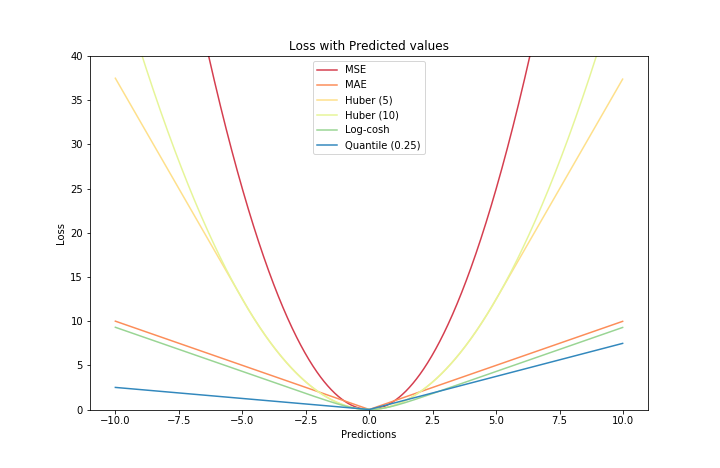
\includegraphics[width=1.0\textwidth]{images/regressions}
    \caption{Common regression losses. \href{https://heartbeat.fritz.ai/5-regression-loss-functions-all-machine-learners-should-know-4fb140e9d4b0}{Source}}
\end{figure}

\subsection{Distributions and Cross Entropy}

Distribution losses are typically used in classification problems, where the task is to build a model $q(x) \mapsto \mathbb{R}^m$ which classifies some 
input $x$ to be in one of $m$ choices. The nominal classification of sample $x$ during training is encoded as a one-hot vector $\hat{y}$, such that $||\hat{y}||_0 = 1$.

Cross-entropy loss takes its foundations from 
information theory. First, we define information as the log-likelihood of some event $x$, based on a given probability distribution:
\begin{align*}
    I(x) = -\log p(x)
\end{align*}
From this definition, we define entropy as the expected value of information given our probability distribution:
\begin{align*}
    \mathbb{E}_{x \sim p}[I] &= \mathbb{E}_{x \sim p} \left[ -\log p(x) \right] \\
    &= -\sum_{x \in p} p(x) \log p(x)
\end{align*}
With this, we can define cross-entropy as the expected value of information in an estimated distribution $q(x)$ over our true distribution $p(x)$:
\begin{align*}
    CE(p || q) &= \mathbb{E}_{x \sim p} \left[ -\log q(x) \right] \\
    &= -\sum_{x \in p} p(x) \log q(x)
\end{align*}

\subsection{Kullback-Leibler Divergence}

Similar to cross entropy, KL-divergence also takes its roots in information theory. Suppose we have a true probability distribution $p(x)$ and we generate 
an estimated distribution $q(x)$, a good measure for the accuracy of our estimated distribution would be to compute the \textit{likelihood ratio} of a given sample 
within the distributions:
\begin{align*}
    LR(p || q)_x = \frac{p(x)}{q(x)}
\end{align*}
Going further, we can compute the likelihood ratio over all samples by taking the product of the likelihood ratios for each samples in our dataset:
\begin{align*}
    LR(p || q) = \prod_{x \in D} \frac{p(x)}{q(x)} = \sum_{x \in D} \log \frac{p(x)}{q(x)}
\end{align*}
With this, we define the KL-Divergence as the expected value of the likelihood ratio over our true distribution $p(x)$:
\begin{align*}
    D_{KL}(p || q) = \mathbb{E}_{x \sim p} \left[ LR(p || q)_x \right] = \sum_{x \in D} p(x) \cdot \log \frac{p(x)}{q(x)}
\end{align*}
It is worth noting that KL-divergence is \textbf{not} a metric because it is not symmetric:
\begin{align*}
    D_{KL}(p || q) \neq D_{KL}(q || p)
\end{align*}
Additionally, KL-divergence does not respect the triangle inequality. \textit{INCOMPLETE.} Shouldn't this be the Cauchy-Schwarz inequality??

Finally, eagle-eyed readers might notice that if $\exists x \in D,\ p(x) > 0,\ q(x) = 0$ then $D_{KL}(p || q) = \infty$. As a result, we typically perform 
\textit{smoothing} to ensure that the sample space of $p$ and $q$ are equal:
\begin{align*}
    \Omega^* &= \Omega(p) \cup \Omega(q) \\
    p^*(x) &= \left.
        \begin{cases}
            p(x) - \frac{|\Omega^* \setminus \Omega(p)|}{|\Omega(p)|} & \text{when } x \in \Omega(p) \\
            \epsilon & \text{otherwise}
        \end{cases}
    \right\} \\
    q^*(x) &= \left.
    \begin{cases}
        q(x) - \frac{|\Omega^* \setminus \Omega(q)|}{|\Omega(q)|} & \text{when } x \in \Omega(q) \\
        \epsilon & \text{otherwise}
    \end{cases}
\right\}
\end{align*}

\textit{INCOMPLETE}. KL divergence as expected value of \href{https://www.countbayesie.com/blog/2017/5/9/kullback-leibler-divergence-explained}{information loss}.

\subsection{Wasserstein Metric} 

The Wasserstein metric originated from the study of optimal transport. 
The metric was used to quantify the amount of work done in the transfer from one mass distribution to another. However, the Wasserstein metric is also 
useful in defining the distance between the spaces of random variables. We will analyse the Wasserstein metric from a 
measure-theoretic perspective, then allude to its applications in deep learning.

Let $(S, d)$ represent a complete, separable metric space and some $0$ in the space (the point chose as $0$ may be arbitrary 
and does not affect of construction here). Suppose $1 \le p < \infty$, then define $\mathfrak{M}_p(S)$ be the collection of 
all probability measures $P$ on the Borel sets of $S$ such that $\int_S d^p(X, 0) dP(X)$ is finite.

Let $\mathfrak{M}_\infty(S)$ be the set of all probability measures on $S$ with bounded support. If $P_1, P_2 \in \mathfrak{M}_p$, then 
the $\ell_p$ Wasserstein distance between $P_1$ and $P_2$ is defined by:
\begin{align*}
    W_p(P_1, P_2) = \left( inf \int d^p(X, Y) d\mu(X, Y) \right)^{\frac{1}{p}}
\end{align*}
Where $\mu$ could be any probability distribution (metric) on the $S \times S$ (this represents the smallest $\sigma$-algebra that contains $S \times S$).
Furthermore, the marginals of this product measure must have marginals $P_1$ and $P_2$.

Further, we define:
\begin{equation}
    W_\infty(P_1, P_2) = inf \| d(X, Y) \|^{(\mu)}_\infty
\end{equation}
Now, we assert that the Wasserstein functions $W_p$ are bona fide metrics on the set $\mathfrak{M}_p$ for $1 \le p \le \infty$ \cite{wass}.

\subsection{Earth Mover's Distance} % INCOMPLETE % formulation then approximation using CDF

In deep learning, we use the Wasserstein-1 metric (technically, an approximation thereof) in multi-class classification problems where there is a notion 
of the distance between proximal models \cite{wassml}. A prime example of this is building a classifier to produce a linear rating (say, 1-10). If the classifier misclassifies 
some example, a distribution loss function like cross-entropy or KL-divergence would only characterize the wrong classification, but not how \textit{far} the predicated label is from 
the true label. With EMD, we don't have this limitation.

If a trained model produces outputs into non-negative, multidimensional space, the we can see the model as a measure. The ground metric here is defined 
as some inherent measure on the feature space. We use the ground metric to establish the Wasserstein metric on the output space. Consider a mapping 
from $\mathcal{X} \in \mathbb{R}^D$ into the space $\mathcal{Y}=R^K_+$ of measures on some finite set $\mathcal{K}$ with $|\mathcal{K}=K|$. 
Then we assume that $\mathcal{K}$ has a ground metric $d_{\mathcal{K}}$, which measures the similarity of output dimensions. 
Further, we learn over some hypothesis space $\mathcal{H}$ of predictors $h_{\theta} : \mathcal{X} \rightarrow \mathcal{Y}$ that is 
parametrized by $\theta \in \Theta$.

We sample independent identically distributed training sample $ = \{ (x_1, y_1), \ldots\, (x_n, y_n)\}$ from some joint distribution 
$\mathcal{P}_{X \times Y}$. Given a measure of performance, $\Sigma$, we want to find the predictor $h_\theta$ that minimizes the 
expected risk, which is $\mathbb{E}[\Sigma(h_\theta(x), y)]$.

Since it's hard to optimize $\Sigma$, we find:
\begin{align*}
    min_{h_\theta \in \mathcal{H}}\Big\{ \mathbb{E}_S\big[ \ell(h_\theta(x), y \big] = \frac{1}{n}\sum_{i=1}^n \ell(h_\theta(x_i), y_i) \Big\}
\end{align*}
Consider a cost function $c: \mathcal{K} \times \mathcal{K} \rightarrow \mathbb{R}$. Then the optimal transport distance to transport the mass in probability measure $\mu_1$ to match that of $\mu_2$ is:
\begin{align*}
    W_c(\mu_1, \mu_2) = inf_{\gamma \in \Pi(\mu_1, \mu_2)} \int_{\mathcal{K} \times \mathcal{K}} c(\kappa_1. \kappa_2)\gamma(d\kappa_1, d\kappa_2)
\end{align*}
We define $\Pi(\mu_1, \mu_2)$ to be the set of joint probability measures on $\mathcal{K} \times \mathcal{K}$ with marginals $\mu_1, \mu_2$.
Now if the cost function is just the metric $d_\mathcal{K}^p$, then this equation is just the Wassertein distance. When $p=1$, we call the metric the Earth Mover's Distance.

In most implementations, EMD loss is not computed exactly because of its computational cost. Instead, we exploit the fact that the EMD is proportional to the difference in the \textit{shapes}
of the distributions. Hence, if we can estimate the difference between the shapes of $p(x)$ and $q(x)$, we would have a loss that scales with the true EMD loss. To quickly estimate the shape of the distributions, 
we use the cumulative distribution function of each distribution:
\begin{align*}
    EMD(p||q) &\approx \sqrt{\sum_{x \in D} \frac{|CDF(p(x)) - CDF(q(x))|^2}{|D|}}
\end{align*}

\pagebreak

%----------------------------------------------------------------------------------------
%	Learning to Learn
%----------------------------------------------------------------------------------------

\section{Learning to Learn: Bayesian Optimization} % hyperparameters

In training a neural network, there are a number of \textit{hyperparameters} that impact the performance of the model. In fact, we have already encountered one: the learning rate for a first order optimizer. There are numerous
other hyperparameters, including the topology of the model for procedural models; the size and amount of data being provided for training; and so on. If we consider the \textit{accuracy} of a model as a function 
of its hyperparameters $\vec{x}$, the task of finding the best model becomes an optimization problem:
\begin{align*}
    \vec{x} \ ^* = \argmin_{\vec{x} \in X} f(x)
\end{align*}
This forms the foundation of the \textbf{meta-learning} field in machine learning. The hyperparameter space is not guaranteed to be differentiatable, hence we are unable to use 
gradient-based numerical optimization methods. We need a bounded black-box global optimizer.

The simplest optimizer to consider is a uniform grid search, where we discretize the hyperparameter space into a grid and evaluate $f(\vec{x})$ at these grid points. The obvious problem with this 
approach is how expensive it becomes, as it suffers gravely from the curse of dimensionality. Instead, we turn to Bayesian optimization.

First, we discuss properties of functions over which we optimize with Bayesian optimization:
\begin{enumerate}
    \item We expect that $f$ is `continuous'. This constraint is a consequence of how we might model $f$ for the optimization. This is a weak constraint;
    if a given basis of the hyperparameter space $X$ is discrete, we can usually make it continuous by encoding it into a one-hot vector $\hat{y}$ such that $||\hat{y}||_0 = 1$. And we can then rediscretize it 
    using a logistic function (like $softmax$) followed by a quantizer.
    \item Following from above, we expect that $X \subset \mathbb{R}^d$, with $d \leq 20$ for best results.
    \item $X$ is a hyperrectangle or simplex in $\mathbb{R}^d$. This is the case as the optimization is typically bounded within some range on each basis of the space.
    \item $f$ is derivative-free, so we cannot use first- or second-order optimization methods on it.
    \item And most importantly, $f$ is expensive to calculate. We are unable to evaluate it enough times in reasonable time to understand its structure.
\end{enumerate}

There are two main components of the Bayesian optimization: an inference model; and a sampling scheme.

\subsection{Building a Surrogate: Gaussian Processes}
In Bayesian optimization, we construct a \textit{surrogate model} for $f$, one which is much easier to evaluate and maximize, and use this surrogate to perform the optimization.
Gaussian Processes (`GP' hereafter) are typically used to model the objective function, although other methods like decision trees might be used. A Gaussian Process is a stochastic 
process such that any finite sub-collection of random variables has a multivariate Gaussian distribution. A stochastic process is an indexed collection of random variables $\{ f(y): y \in Y \}$ where 
$Y$ is the index set. Essentially, a Gaussian Process describes a \textit{distribution over functions} in the domain $X$.

For a 1D parameter space, we designate the distribution $\{ f(x) |\ x \in X \}$ where the value $f(x) \sim \mathcal{N}(\mu(x), \sigma(x, x'))$, where $\mu(x)$ is the mean of $f$ over $X$ and $\sigma(x, x')$ is the covariance kernel
of the Guassian Process that determines the linkages between different points in the domain.

\textit{INCOMPLETE}. Diagram showing distribution of functions.

We apply Bayesian Inference to the Gaussian Process:
\begin{align*}
    \text{posterior} \propto (\text{prior} \times \text{likelihood})
\end{align*}
Which is given in closed form when using a Gaussian Process. We construct a mean vector by evaluating the mean function at each $x_i$ and a covariance matrix by [pairwise evaluating kernel]?? Doing this at $k$ points, we have a prior on:
\begin{align*}
    f(x_{1:k}) \sim \mathcal{N}(\mu_0(x_{1:k}), \Sigma_0(x_{1:k}, x_{1:k}))
\end{align*}
With this, we have an updated posterior upon evaluation of a new $x$, $f(x)$:
\begin{align*}
    f(x) |\ f(x_{1:n}) \sim \mathcal{N}(\mu_n(x), \sigma^2_n(x))
\end{align*}
Where:
\begin{align*}
    \mu_n(x) &= \Sigma_0(x, x_{1:n}) \Sigma_0(x_{1:n}, x_{1:n})^{-1} \left( f(x_{1:n}) - \mu_0(x_{1:n}) \right) + \mu_0 \\
    \sigma_n^2(x) &= \Sigma_0(x, x) - \Sigma_0(x, x_{1:n}) \Sigma_0(x_{1:n}, x_{1:n})^{-1} \Sigma_0(x_{1:n}, x)
\end{align*}
Where $\Sigma_0$ is the covariance matrix. Hence with this, we have a closed-form solution for Bayesian updates. However, there is a multitude of considerations to make when choosing 
a \textit{covariance kernel}, which determines $\Sigma_0$.

\pagebreak

\subsection{Common Covariance Kernels}
We want to choose a covariance kernel $K(x_i, x_j)$ which has the following properties:
\begin{enumerate}
    \item \textbf{Stationary}. We say that $K(x_i, x_j)$ is stationary if $K(x_i, x_j) = g(x_i - x_j)$ where $g$ is an arbitrary function. This property guarantees 
    translational invariance of the kernel.

    \item \textbf{Isotropic}. We say that $K(x_i, x_j)$ is stationary if $K(x_i, x_j) = g(|x_i - x_j|)$ where $g$ is an arbitrary function. This property guarantees 
    rigid motion invariance of the kernel.

    \item \textbf{Semi-Positive Definiteness}. The Gram Matrix $G_{i,j} = K(x_i, x_j)$ must be such that $\forall \vec{v} \in \mathbb{R}^n,\ \vec{v}^T G \vec{v} \geq 0$ with $G \in \mathbb{R}^{n \times n}$.
\end{enumerate}

\subsubsection{Squared Exponential Kernel}
\begin{align*}
    K_{\text{SE}}(x_i, x_j) = \exp \left( -\frac{(x_i - x_j)^2}{2l^2} \right)
\end{align*}
Where $l$ defines the length scale. As $l >> 0$, the correlation of distant values increases and the graph becomes smoother:

\textit{INCOMPLETE}. Diagram here.

Some argue that the squared-exponential covariance kernel is too idealistic, and that a rougher shape would be more representative of real-world phenomena. Hence the motivation for the Matern kernel.

\subsubsection{Matern Kernel}
\begin{align*}
    K_{\text{Matern}}(x_i, x_j) = \frac{2^{1-v}}{\Gamma(v)} \left( \sqrt{2v} \frac{|x_i - x_j|}{\rho} \right)^v K_v \left( \sqrt{2v} \frac{|x_i - x_j|}{\rho} \right)
\end{align*}
Where $v$ and $\rho$ are positive parameters, $\Gamma$ is the gamma function, and $K_v$ is a Weber function (a Bessel function of the second kind). $v$ is usually any $p + \frac{1}{2},\ p \in \mathbb{Z}^+$.
As $v \rightarrow \infty$, the function becomes smoother. Setting $v = \frac{1}{2}$, $K_{\text{Matern}}(x_i, x_j) = \exp(-\frac{|x_i - x_j|}{\rho})$. This opens up the $\gamma$-class of covariance functions:
\begin{align*}
    K_\gamma (x_i, x_j) = \exp \left( -\left(\frac{|x_i, x_j|}{\rho} \right)^\gamma \right) \text{ for } 0 < \gamma \leq 2
\end{align*}

\subsection{Kernels and Hyper-hyper Parameter Optimization}
The task of choosing a suitable kernel for covairance is itself somewhat of an optimization problem. In this section, we discuss some considerations.

First, we need a good metric on which to measure the performance of the kernel. An important metric to use is \textbf{generalization error}. This is a measure of how well 
the model will be able to generalize to unseen data. The kernel that performs best with respect to this metric is usually the most optimal choice for a Gaussian Process.

Once a covariance kernel is chosen, there are usually hyperparameters which affect the performance of the model. For the squared-exponent kernel, the sole hyperparameter is the length scale $l$. For the 
Mattern kernel, there are $v$, $\rho$. We usually use a \textbf{maximum a-posteriori} probability estimate (`MAP' estimate):
\begin{align*}
    \eta^* = \argmax_\eta P(f(x_{1:n}) |\ \eta)
\end{align*}
Where $\eta$ is the kernel's hyperparameters. The MAP estimate gives us the maximum for the data we have.

\subsection{Exploration and Exploitation: The Acquisition Function}
We have explored how to build and update the surrogate model using Bayesian inference. The other half of the Bayesian Optimization process is finding a scheme to sample the objective function, with which we can use the samples to 
update our surrogate and optimize. To do so, we use an \textbf{Acquisition Function} which provides proposals for new samples to take. The choice of acquisition function is made with the central consideration of 
balancing of \textbf{exploration and exploitation}.

We want an acquisition function that explores the objective landscape, as doing so increases chances of finding a global minimum. On the other hand, we want the acquisition function to also exploit already-explored regions 
to find proximal maxima.

\subsubsection{Expected Improvement}
Expected Improvement is a common choice for an acquisition function. First, we assume that we have taken $n$ samples of the objective function $f(x)$. Let $f(x^*)$ be the maximum over $n$ samples. We then consider the 
utility of our prospective sample as:
\begin{align*}
    u(x) = (f(x) - f(x^*))^+
\end{align*}
The expected value of $u(x)$ provided data is given in closed form based on the Gaussian Process model:
\begin{align*}
    EI(x) &= \mathbb{E}\left[ u(x) |\ x_{1:n}, f(x_{1:n}) \right] \\
    x_{EI}^* &= \argmax_{x \in X} EI(x)
\end{align*}

\subsubsection{Knowledge Gradient}
Given $n$ observations of $f(x)$, Expected Improvement assumes that the maximum exists within those points. In this, EI assumes that the objective is noise-free and uses a risk-averse policy. Knowledge Gradient however does not make these 
assumptions:
\begin{align*}
    KG_n(x) &= \mathbb{E}_n \left[ \mu_{n+1}^* - \mu_n^* |\ x_{n+1} = x \right] \\
    x_{KG}^* &= \argmax_{x \in X} KG(x)
\end{align*}
The Knowledge Gradient acquisition function focuses on improving the GP model to accurately model the underlying objective $f(x)$. In this sense, Knowledge Gradient prioritizes exploration of the 
objective landscape as opposed to exploitation of already-visited regions.

\pagebreak

\subsection{Inference and Markov Chain Monte Carlo}

Going beyond Bayesian Optimization, a fundamental problem we face is the task of estimating the geometry of a distribution. In Bayesian Optimization, we achieve this by utilizing value heuristics within acquisition functions. In Bayesian Inference, this 
task is central in computing a posterior given an observation.

For some distribution $D$ over a finite set $X$, in which we know $p(x)$ for $x \in X$ but not the geometry of the distribution, we can use the Markov Chain Monte Carlo method to approximate this distribution. First, we introduce the Monte Carlo sampling method.

\subsubsection{Monte Carlo Sampling}

We define some multi-dimensional space $X$ with some density $p(x)$ defined on it. First consider the samples $\{x^1, \ldots, x^N\}$ drawn from independent, 
identical distributions (i.i.d). The Monte Carlo method to approximate this density is to define the point-mass function:
\begin{align}
    p_N(x)=\frac{1}{N}\sum_{i=1}^{N}\delta_{x^{(i)}}(x)
\end{align}
Where $\delta_{x^{(i)}}(x)$ is the Dirac-delta function. We have:
\begin{align}
    I_N(f)=\frac{1}{N}\sum_{i=1}^{N}f(x^{i}) \xrightarrow{a.s.} I(f) = \int_X f(x)p(x)dx
\end{align}
Where $a.s.$ means "almost surely" in a measure-theoretic sense. Equation (4.2) is correct under the assumption that the sampling is unbiased and extenseive with respect to the Law of Large Numbers.
One might also analyze the error with the Central Limit Theorem for the convergence to the integral.
Notice that if we consider an integral of $f$ over $D \subset \mathbb{R}^n$, then we can use this approach to solve for the 
integral of $f$\footnote{This method is very different from techniques such as the Simpson's rule because it is non-deterministic}. Observe:
\begin{align*}
    \int_D f(x) \frac{1}{V(D)} dx = \lim_{N \rightarrow \infty} \frac{V(D)}{N} \sum_{i=1}^{N} f(x^{(i)})
\end{align*}
Where $V(D)$ is the volume of the domain $D \in \mathbb{R}^n$ and we assume $p(X)$ is the uniform distribution over $D$. This defines the vanilla Monte Carlo sampling method. Because the method becomes 
inefficient and intractable as $\dim X >> 0$, we introduce a sampling heuristic to make the method more tractable.

\subsubsection{Rejection Sampling}
Suppose we had a distribution $q(x)$ also on $X$ where $p(x) \le Mq(x)$ for some $M < \infty$ for all $x \in X$. 
Starting as some point $x_{(1)} \in X$, we sample $q(x^*)$ from a proposal $x^*$. If we accept $x^*$, 
then we set $x_{(2)} = x^*$. And if we reject it, we keep $x_{(2)} = x_{(1)}$.
This gives us a simple iteration scheme: \\[0.5cm]
\begin{algorithm}[H]
    \caption{Rejection Sampling}
    \SetAlgoLined
    \KwResult{sample set $\{x_{(i)}\}$}
        \While{$i < N$} {
            Sample $x^*$ from $q(x)$ and $u$ from $\mathcal{U}_{(0,1)}$ \:
            
            \eIf{$u < \frac{p(x^*)}{Mq(x^*)}$
            }{
                $x_{(i)} = x^*$ \par
                accept
            }{
                reject
            }\
        }
\end{algorithm}
Rejection sampling can be impractical because we may not be able to find an efficient $q(x)$. For instance, 
if the constant factor $M$ is very large, then the acceptance rate of the algorithm 
will be very low. As a consequence, the rate of convergence would be too slow for 
practical purposes:
\begin{align*}
    Pr(x \text{ accepted}) = Pr\Big(u < \frac{p(x)}{Mq(x)} \Big) = \frac{1}{M}
\end{align*}
As $M$ increases, the probability of acceptance decreases in inverse proportionally.
\begin{figure}[H]
    \centering
    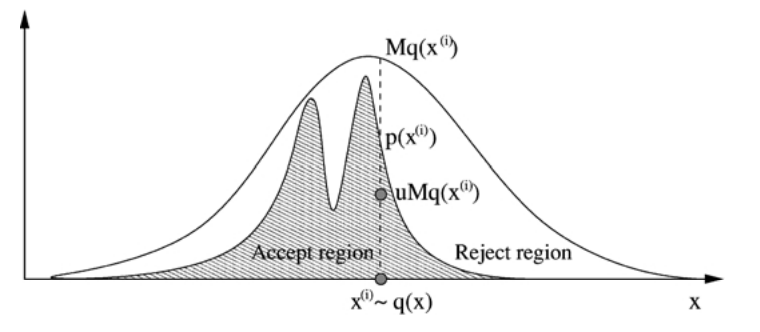
\includegraphics[width=0.7\textwidth]{images/rejection}
    \caption{\text{Rejection sampling example, Andrieu et al.}}
\end{figure}

\pagebreak

%----------------------------------------------------------------------------------------
%	Understanding Data
%----------------------------------------------------------------------------------------

\section{Understanding Data: Spectral Analysis}

What is your favorite song? You probably listen to it while studying or running, singing along
while bopping your head. If asked to identify what you like about it, you might mention the artiste's voice 
or the instrumental. But how can you tell apart different aspects of the song? Afterall, what you hear 
is really just the sum of all sounds, losing information about which sound is which.

In this chapter, we will explore spectral analysis starting with 1D signals (sounds) before looking at different 
applications thereof in deep learning. But first, let us explore the nature of signals and how we digitize them.

\subsection{Characterizing Signals}

\begin{itemize}
    \item Continuous signals
    \item Discretization by fixed-interval sampling
    \item Nyquist-Shannon sampling theorem
    \item Audio, air pressure, and microphones
    \item Expanding to n-D signals: images
\end{itemize}

\subsection{Discrete Fourier Transform}

\begin{itemize}
    \item Fourier synthesis:
    \begin{align*}
        \mathcal{F}(x, f) &= \int_{-\infty}^{\infty} x(t) \cdot \exp \left( -2 \pi i f t \right) dt \\
        \mathcal{F}(x, f) &= \sum_{t=1}^{N} x(t) \cdot \exp \left( \frac{-2 \pi i f t }{N} \right)
    \end{align*}
    \item The DFT is a complex transform
    \item Continuous formulation then discrete
    \item Amplitude and phase spectra
\end{itemize}

\begin{figure}[H]
    \centering
    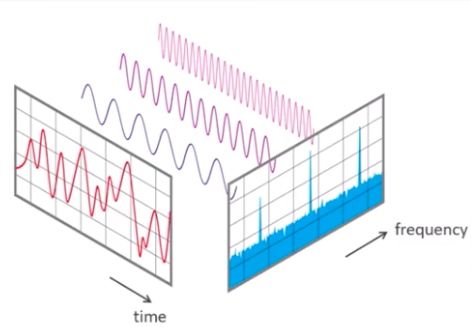
\includegraphics[width=0.65\textwidth]{images/freq}
    \caption{Frequency Transform. \href{https://towardsdatascience.com/fourier-transformation-and-its-mathematics-fff54a6f6659}{Source}}
\end{figure}

\subsection{Short-Time Fourier Transform}

\begin{itemize}
    \item Formulation:
    \begin{align*}
        STFT(x, f, \tau) = \int_{-\infty}^{\infty} \left( x(t) \cdot \omega^*(t - \tau) \right) \cdot \exp \left( -2 \pi i f t \right) dt
    \end{align*}
    \item We can choose $\omega(t)$ to be Gaussian, square, triangular, or others. Look at \href{https://en.wikipedia.org/wiki/Window_function}{window functions}.
    \item Non-stationary signals, Heinsberg uncertainty and STFT
    \item Assume signal is stationary over some small interval, a.k.a window is \textit{compactly supported}.
    \item Use of small window means less frequency resolution, and use of large window means less temporal resolution.
\end{itemize}

\subsection{Discrete Wavelet Transform}

\begin{itemize}
    \item The need for better temporal resolution than STFT. We need a multi-resolution transform.
    \item Problem with STFT is that if the window is a scaled dirac pulse, then we are really performing 
    FFT of convolution of signal and dirac pulse. But this means we are taking the product of FFT of dirac pulse and 
    FFT of signal. The problem is that FFT of dirac pulse is spread over all frequencies. Hence we get spectral leaking.
    \item Formulation:
    \begin{align*}
        \Psi(x, \tau, s)_\psi = \frac{1}{\sqrt{|s|}} \int_{-\infty}^{\infty} x(t) \cdot \psi^* \left( \frac{t  - \tau}{s}  \right) dt
    \end{align*}
    Where $\tau$ is translation (offset), $s$ is scale, and $\psi$ is \textbf{mother wavelet}.
    \item Basis functions (wavelets) are compactly supported, periodic functions.
    \item Typically, $\displaystyle s = \frac{1}{f}$
    \item Admissibility condition. The fourier transform of the mother wavelet must be zero at zero frequency.
    \item Haar wavelet, Mexican hat wavelet as 2nd derivative of the Gaussian
    \item Discretization by applying Nyquist-Shannon on sampling grid, dyadic sampling.
\end{itemize}

\subsection{Applications in Deep Learning}

\subsubsection{Images and Convolutions}

\begin{itemize}
    \item For a 2D image:
    \begin{align*}
        \mathcal{F}(x)_{(k, l)} = \sum_{a = 1}^N \sum_{b = 1}^N f(a, b) \cdot \exp \left( -2 \pi i \left( \frac{ka}{N} + \frac{lb}{N} \right) \right)
    \end{align*}
    \item Convolution theorem for fourier transform
    \item Direct convolution vs FFT convolution
    \item cuFFT
\end{itemize}

\subsubsection{Audio and Spectrograms}

\begin{itemize}
    \item Audio mixing and remixing
    \item Raw audio analysis with CNN. Spectrogram using STFT.
\end{itemize}

\pagebreak

%----------------------------------------------------------------------------------------
%	Understanding Datasets
%----------------------------------------------------------------------------------------

\section{Understanding Datasets: Bayes Error}

\pagebreak

%----------------------------------------------------------------------------------------
%   References
%----------------------------------------------------------------------------------------

\begin{thebibliography}{999}

    \bibitem{vcdim}
        Blumer, A. et. al (1989).
        \emph{\href{http://www.trhvidsten.com/docs/classics/Blumer-1989.pdf}{Learnability and the Vapnik-Chervonenkis Dimension }}.

    \bibitem{cortex}
        Kuzovkin, I., Vicente, R., Petton, M. et al. (2018).
        \emph{\href{https://www.nature.com/articles/s42003-018-0110-y}{Activations of deep convolutional neural networks are aligned with gamma band activity of human visual cortex}}

    \bibitem{batchnorm}
        Ioffe \& Szegedy (2015).
        \emph{\href{https://arxiv.org/abs/1502.03167}{Batch Normalization: Accelerating Deep Network Training by Reducing Internal Covariate Shift}}.

    \bibitem{instancenorm}
        Ulyanov, Vedaldi, \& Lempitsky (2016).
        \emph{\href{https://arxiv.org/abs/1607.08022}{Instance Normalization: The Missing Ingredient for Fast Stylization}}

    \bibitem{wgangp}
        Gulrajani et. al. (2017).
        \emph{\href{https://arxiv.org/abs/1607.08022}{Improved Training of Wasserstein GANs}}.

    \bibitem{wassml}
        Frogner et al. (2015).
        \emph{\href{https://arxiv.org/abs/1506.05439}{Learning with a Wasserstein Loss}}

    \bibitem{wass}
        Givens, Shortt. (1984).
        \emph{\href{https://projecteuclid.org/download/pdf_1/euclid.mmj/1029003026}{A Class of Wasserstein Metrics for Probability Distributions}}

\end{thebibliography}

\vfill

%----------------------------------------------------------------------------------------

\end{document}
